%===================================================================================
\subsection{CU31 Ver avances commit}
{
\justify
\color{blue}{\textbf{Objetivo}}
}

%------------------------------------------------------------------
\justify
Permitir al Lider de proyecto y al colaborador, ver los detalles del avance del commit.
%------------------------------------------------------------------
{
\justify
\color{blue}{\textbf{Diseño}}
}
%-------------------------------------------------------------------------------
\justify
En la figura \ref{fig:IU31} se muestra la pantalla, en donde Permitir al Lider de proyecto y al colaborador, ver los detalles del avance del commit.

\begin{figure}[htb]
\centering
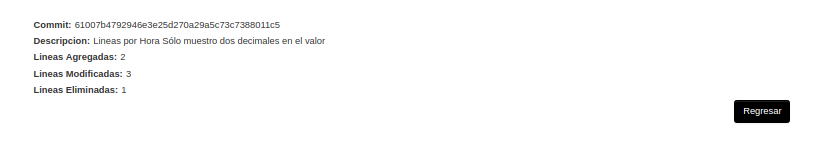
\includegraphics[width=0.8\textwidth]{./images/cu31-avance-commit.png}
\caption{Ver estadisticas de avances de las tareas.} \label{fig:IU31}
\end{figure}

\newpage